\documentclass[12pt]{article}
\usepackage[margin=1cm, bottom=2cm, portrait, a4paper]{geometry}
\usepackage{indentfirst}
\usepackage{graphicx}
\usepackage{fontspec}
\usepackage{amsmath}
\usepackage{mathtools}

\title{Информационные технологии. Лекция 10. SLAM}
\author{Студент группы 2305 Макурин Александр}
\date{24 апреля 2023}

\setmainfont[Ligatures=TeX]{Linux Libertine}
\graphicspath{./graphics/}

\begin{document}
\maketitle
$S = \{S_1, ..., S_T\}$ — положение относительно того, что видит объект.

$z = \{z_1, ..., z_T\}$ — объекты (роботы).

$M$ — общая карта.

$X = \{X_1, ..., X_T\}$ — наблюдения над посторонними объектами.

$\overline{S} = \{\overline{S_1}, ..., \overline{S_T}\}$ — положение с учётом $S$, $z$, $M$. $S_i = f(S, z, M)$.

\section{Полный (Full) SLAM}

$[\overline{S_{t-1}}, \overline{S_t}, \overline{S_{t + 1}}]$ — хотим построить.

$[z_{t - 1}, z_t, z_{t+1}]$ — объекты, то, что видит объект.

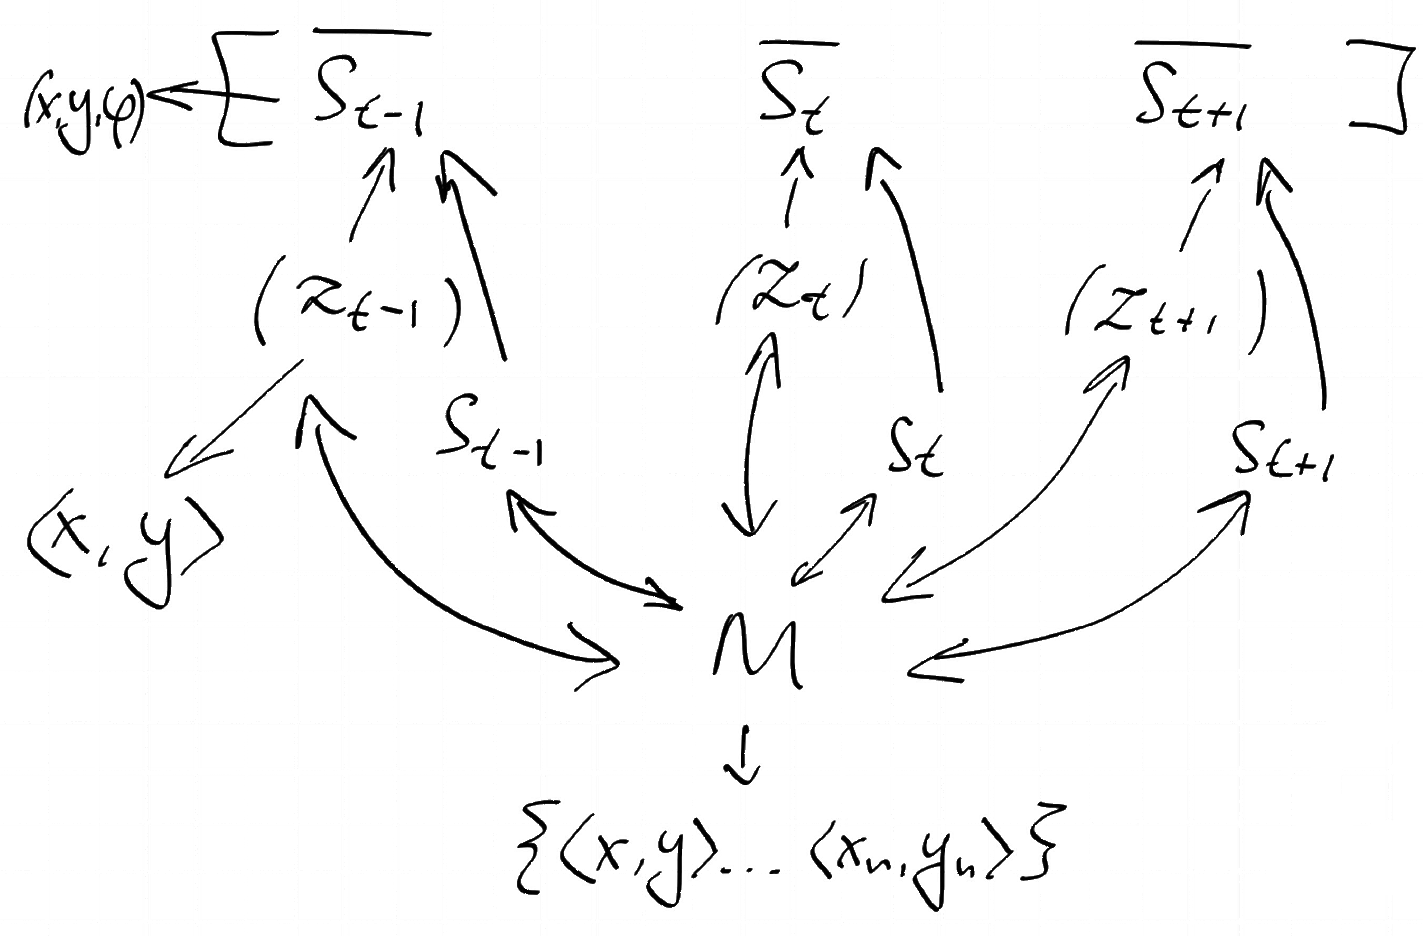
\includegraphics[width=0.5\textwidth]{graphics/pic01.png}

$z_j = z_j^{\text{изв.}} \cup z_j^{\text{неиз.}}$

$S_{t-1} \xrightarrow{U = <V, \phi>} S_t$

$P(\overline{S}, M|S, z)$ — вероятность нахожения в точке $\overline{S}$. В данном случае будет множество вероятностей для множества точек ($|P|=|S|$).

$t_i$:

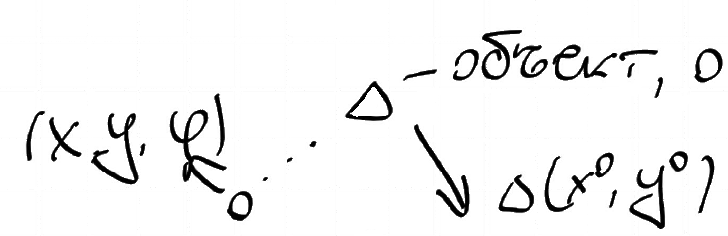
\includegraphics[height=0.1\textheight]{graphics/pic02.png}

$t_{i+1}$:

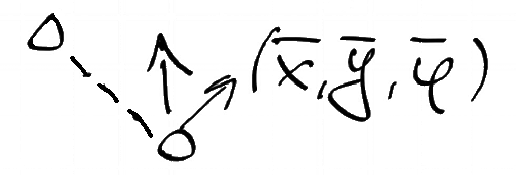
\includegraphics[height=0.1\textheight]{graphics/pic03.png}

\section{Online SLAM}

Определение положения в конкретный момент времени: $P(\overline{S_T}, M|S, z) \Rightarrow \int ... \int P(\overline{S}, M|S, z) d\overline{S_i} ... d \overline{S_n}$.

EKF — Extended Kalman Filter.

\section{EKF-SLAM}
\subsection{Этап 1}

$S_i = [x_i, y_i, \phi_i]$ — состояние системы в данный момент.

$P_S = \begin{bmatrix}
        \delta_{xx}^2     & \delta_{xy}^2     & \delta_{x\phi}^2     \\
        \delta_{yx}^2     & \delta_{yy}^2     & \delta_{y\phi}^2     \\
        \delta_{\phi x}^2 & \delta_{\phi y}^2 & \delta_{\phi \phi}^2 \\
    \end{bmatrix}$ — матрица отклонения. $\delta_{yx}^2$ — насколько ошибается $y$ при изменении $x$.

$Env = \{<x_0, y_0>, ..., <x_n, y_n>\}$

$P_{Env} = \begin{bmatrix}
        \delta_{x_0x_1}^2 & \delta_{x_0y_0}^2 &                   \\
                          & \delta_{y_0y_0}^2 &                   \\
                          &                   & \delta_{x_1x_0}^2 \\
    \end{bmatrix}$

$X = [S, Env]$ — где находимся относительно других объектов.

$P =\begin{bmatrix}
        P_S        & P_{SEnv} \\
        P^T_{SEnv} & P_{Env}
    \end{bmatrix}$

$P_{SEnv}$ — $P_{Env}$ дополненная нашим объектом (его отклонение относительно других).

$P_{SEnv} = 2\begin{bmatrix}
        \delta^2_{xx_0} & \delta^2_{xy_0} & \delta^2_{xx_1} & ... \\
        \delta^2_{yx_0} & \delta^2_{yy_0} & \delta^2_{yx_1} & ... \\
    \end{bmatrix}$

$P_S \neq 0$, $P_{Env} \neq 0$

$U$ — управляющее воздействие. Задача — понять местоположение на основании одометрии и $U$.

$\overline{S_i} = \begin{bmatrix}
        f(\overline{S_{i-1}}, U) \\
        S_i
    \end{bmatrix}$, где $S_i$ — собственный анализ происходящего.

$P_i = \begin{bmatrix}
        \nabla g P_{i - 1} \nabla g^T + Q & \nabla g P_{i-1}^0 \\
        (\nabla g \cdot P_{i - 1}^0)^T    & P_{i - 1}^0
    \end{bmatrix}$ — ошибка измерений относительно объекта \\
$\nabla g = \dfrac{\delta f}{\delta x}$ — динамики относительно координат \\
$Q = \nabla g_U U \nabla g_U^T$ — шум процесса (динамика относительно управляющего воздействия) \\
$\nabla g_U = \dfrac{\delta f}{\delta V}$ \\
$\nabla g P_{i - 1} \nabla g^T$ — шум позиции \\
$\nabla g P_{i-1}^0$ — оценка положения ориентиров с учётом шума положения робота

$U = \begin{bmatrix}\delta^2_x & 0 \\ 0 & \delta^2_U\end{bmatrix}$

Новые координаты основаны на известных старых и рассчёте нового шума с учётом старого.

\subsubsection{EKF. Общие алгоритмы}
\begin{enumerate}
    \setcounter{enumi}{-1}
    \item Инициализация
    \item Оценка собственного местоположения (мп) ($S$)
    \item Оценка мп ориентиров ($\widetilde{S}$)
    \item Оценка мп новых объектов ($\overline{S}$)
    \item Конец ($M$)
\end{enumerate}

\subsection{Этап 2}
$x_i = [\rho, \theta]$

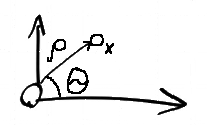
\includegraphics[height=0.1\textheight]{graphics/pic04.png}

$h_i = \begin{bmatrix}
        \sqrt{(x_i - x^S)^2 - (y_i - y^S)^2} \\ \arctan (\dfrac{y_i - y}{x_i - x} - \phi^S)
    \end{bmatrix}$

$\nu_i = h_i - x_i$

$H = \nabla h P_i \nabla h^T + R$

$\nabla h = \dfrac{\delta h}{\delta S}$

$R = \begin{bmatrix}\delta_\rho^2 & 0 \\ 0 & \delta_\theta^2\end{bmatrix}$ — матрица ошибок относительно $\rho$. $\delta^2_\rho$ — насколько неверно оценено мп объектов

$X \xrightarrow{\text{Уточнение на основе $H$}} \overline{X}$

$\omega = P \nabla h^T H^{-1} + R$ — коэффициент усиления Калмана. Показывает насколько должны учитываться отклонения.

$\overline{S_i} = S_i + \omega_i \nu_i$

$\overline{P_i} = P_i - \omega_i H \omega_i^T$

В результате имеем информацию о мп ориентиров.

\subsection{Этап 3}

$x_i^0 = \begin{bmatrix} \overline{S_i} \\ f(S_i, z_i) \end{bmatrix}$

$P_i = \begin{bmatrix}P_i & P_{i0} \\ P_{i0}^T & P_i^0\end{bmatrix}$ — шум, $P_{i0}$ — шум положения робота относительно объекта.

$P_i = \begin{bmatrix}
        P_i            & P_{i0}           & P_i \nabla g_x                                            \\
        P_{i0}^T       & P_i^0            & P_i^0 \nabla g_x                                          \\
        \nabla g_x P_i & \nabla g_x P_i^0 & \nabla g_x P_i \nabla g_x^T + \nabla g_x^0 R \nabla g_x^T
    \end{bmatrix}$

$\nabla g_x = \dfrac{\delta f}{\delta x}$ — динамика изменения состояния объекта

$\nabla g_x^0 = \dfrac{\delta f}{\delta x^0}$
$\nabla g_x = \dfrac{\delta f}{\delta x}$

В итоге формируем новый $\overline{z_i}$ и составляем карту $M$.

В Fast SLAM пропадает $\nabla g_x^0$, $P_i^0 = 0$. $x^0 = x + \rho(z_i)$.

Сложность растёт очень сильно при росте количества взаимозависимых в пространстве объектов.

$P(S|U,z) = P(V|U, z) \cdot \prod P(M | U,z,V)$

\subsection{Требования к ориентирам:}

\begin{enumerate}
    \item Уникальность
    \item Возможность получить информацию о нём из нескольких точек\
    \item Статичность
    \item Изобильность — ориентиров должно быть достаточно
\end{enumerate}

\end{document}